\section{MIP on arbitrary polygonal cells} \label{sec_mip}
\subsection{PWLD finite elements}
In this section, we introduce the PieceWise Linear Discontinuous (PWLD) finite
elements developed in \cite{pwld_2d,pwld_3d}. To obtain the PWLD basis
functions on two-dimensional polygons, we need to introduce the within-cell
point $c$. The coordinates of $c$ are weighted averages of the vertex coordinates:
\begin{align}
& x_c = \sum_{j=1}^{V} \alpha_{j} x_j\\
& y_c = \sum_{j=1}^{V} \alpha_{j} y_j
\end{align}
where $\sum_{j=1}^{V} \alpha_{j}=1$, $\alpha_j \geq 0\ \forall j$, and $V$ is 
the number of vertices of the cell.\\
The basis function at vertex $j$ is defined by \cite{pwld_2d}:
\begin{equation}
b_{j} (x,y) = t_{j}(x,y) + \alpha_j t_c(x,y)
\end{equation}
where the $t_j$ functions are the linear functions on the triangle formed
by the three vertices $j-1$, $j$ and $j+1$: $t_j (x,y)$ is unity at vertex $j$
and zero at $j-1$ and $j+1$. The function $t_c(x,y)$ is unity at $c$ 
and zero at each vertex. In this paper, the arbitrary positive weights
$\alpha_j$ are chosen to be $\frac{1}{V}$. On a square cell with 
$\alpha_{j}=0.25\ \forall j$, the basis functions are given in Figure (\ref{pwld}):
\begin{figure}[H]
\centering
\subfloat[First basis function]{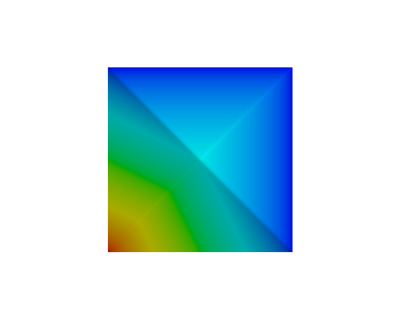
\includegraphics[width=0.3\textwidth]{pwld_1}}
\subfloat[Second basis function]{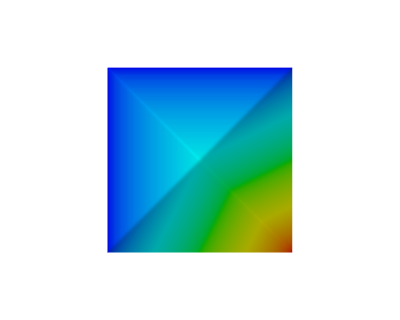
\includegraphics[width=0.3\textwidth]{pwld_2}}\\
\subfloat[Third basis function]{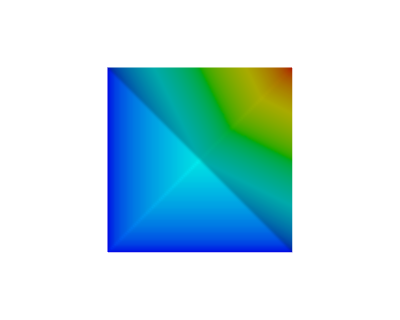
\includegraphics[width=0.3\textwidth]{pwld_3}}
\subfloat[Fourth basis function]{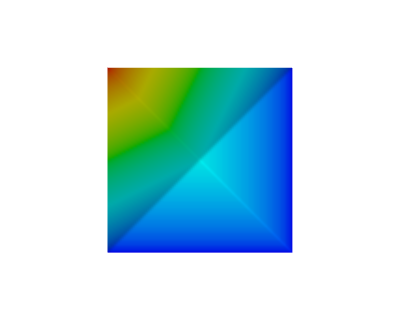
\includegraphics[width=0.3\textwidth]{pwld_4}}
\caption{PWLD basis function}
\label{pwld}
\end{figure}
On triangular cells, the PWLD basis functions reduces to the standard Linear
Discontinuous (LD) basis functions if $\alpha_j = \frac{1}{3}$. Given the 
definition of the PWLD finite elements, it may seem complicated to build the 
mass matrix or the gradient matrix on an arbitrary polygonal cells but the 
construction of such matrices can be greatly simplified using ``side'' sub-cells. 
A ``side'' sub-cell is a triangular cell made from two adjacent vertices and the 
point $c$. On each ``side'' sub-cells the mass matrix, for example, can be build
using LD finite elements. The coefficients in the matrix correspondent to the 
point $c$ are shared among the basis function in the cell. For instance the
mass matrix associated to a quadrilateral cell can be built as follows:\\
First let us define the mass matrix, $\bs{M}_{PWLD}$, and the mass matrix on a 
``side'' sub-cell $\bs{M}_S$. We assume that the third basis function is associated 
to the middle point of the cell. The first (respectively second) basis function on 
the cell correspond to the first (respectively second) basis function of the 
``side'' sub-cell.
\begin{figure}[H]
  \centering
  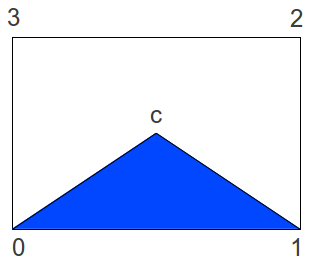
\includegraphics[width=0.3\textwidth]{mass_matrix}
  \caption{Sub-cell in the cell}
\end{figure}
Now, $\bs{M}_{PWLD}$ can be filled in using $\bs{M}_S$:
{\allowdisplaybreaks
\begin{align}
  & \bs{M}_{PWLD}(0,0) =  \bs{M}_S(0,0) + \alpha \bs{M}_S(0,2) + \alpha
  \bs{M}_S(2,0) + \alpha^2 \bs{M}_S(2,2)\\
  & \bs{M}_{PWLD}(0,1) =  \bs{M}_S(0,1) + \alpha \bs{M}_S(0,2) + \alpha
  \bs{M}_S(2,1) + \alpha^2 \bs{M}_S(2,2)\\
  & \bs{M}_{PWLD}(0,2) =  \alpha \bs{M}_S(0,2) + \alpha^2 \bs{M}_S(2,2)\\
  & \bs{M}_{PWLD}(0,3) =  \alpha \bs{M}_S(0,2) + \alpha^2 \bs{M}_S(2,2)\\
  & \bs{M}_{PWLD}(1,0) =  \bs{M}_S(1,0) + \alpha \bs{M}_S(1,2) + \alpha
  \bs{M}_S(2,0) + \alpha^2 \bs{M}_S(2,2)\\
  & \bs{M}_{PWLD}(1,1) =  \bs{M}_S(1,1) + \alpha \bs{M}_S(1,2) + \alpha
  \bs{M}_S(2,1) + \alpha^2 \bs{M}_S(2,2)\\
  & \bs{M}_{PWLD}(1,2) =  \alpha \bs{M}_S(1,2) + \alpha^2 \bs{M}_S(2,2)\\
  & \bs{M}_{PWLD}(1,3) =  \alpha \bs{M}_S(1,2) + \alpha^2 \bs{M}_S(2,2)\\
  & \bs{M}_{PWLD}(2,0) =  \alpha \bs{M}_S(2,0) + \alpha^2 \bs{M}_S(2,2)\\
  & \bs{M}_{PWLD}(2,1) =  \alpha \bs{M}_S(2,1) + \alpha^2 \bs{M}_S(2,2)\\
  & \bs{M}_{PWLD}(2,2) =  \alpha^2 \bs{M}_S(2,2)\\
  & \bs{M}_{PWLD}(2,3) =  \alpha^2 \bs{M}_S(2,2)\\
  & \bs{M}_{PWLD}(3,0) =  \alpha \bs{M}_S(2,0) + \alpha^2 \bs{M}_S(2,2)\\
  & \bs{M}_{PWLD}(3,1) =  \alpha \bs{M}_S(2,1) + \alpha^2 \bs{M}_S(2,2)\\
  & \bs{M}_{PWLD}(3,2) =  \alpha^2 \bs{M}_S(2,2)\\
  & \bs{M}_{PWLD}(3,3) =  \alpha^2 \bs{M}_S(2,2)
\end{align}}    
By looping over all the ``side'' sub-cell of a cell, the mass matrix of the 
cell can be easily built.
\subsection{Modified Interior Penalty DSA}
The transport equation can be written in a compact form using operators:
\begin{align}
  &\bs{L} \psi = \bs{M}\bs{\Sigma} \phi + Q \label{transport}\\
  &\phi = \bs{D}\psi \label{phi_D_psi}
\end{align}
where $\psi$ are the angular fluxes, $\phi$ are the moments of the flux, $Q$
is the volumetric source, $\bs{L}$ is the streaming operator, $\bs{M}$ is the
moments-to-directions operator and $\bs{D}$ is the directions-to-moments
operator. \Cref{transport,phi_D_psi} can be solved using the Source Iteration 
(SI) method, which is a Richardson iteration. The Source Iteration method at 
the $k^{th}$ iteration is given by:
\begin{equation}
\phi^{(k+1)} = \bs{DL}^{-1} \bs{M\Sigma}\phi^{(k)}+\bs{DL}^{-1}Q
\end{equation}
When the scattering ratio $c = \frac{\Sigma_s}{\Sigma_t}$ tends to one, with 
$\Sigma_s$ the scattering cross section and $\Sigma_t$ the total cross section, 
the spectral radius of SI can become arbitrary close to one.  In
this case, DSA can be used to accelerate the convergence which otherwise
would be very slow. The SI+DSA  scheme is given by a transport sweep:
\begin{equation}
\phi^{(k+1/2)} = \bs{DL}^{-1}\bs{M\Sigma}\phi^{(k)} +\bs{DL}^{-1}Q,
\label{dsa_sweep}
\end{equation}
followed by a diffusion synthetic acceleration for the correction:
\begin{equation}
\delta \phi^{(k)} = \bs{\mc{T}}^{-1} \bs{R} \(\phi^{(k+1/2)}-\phi^{(k)}\),
\label{correction}
\end{equation}
yielding the next iterate for the flux moments:
\begin{equation}
\phi^{(k+1)} = \phi^{(k+1/2)} + \bs{P} \delta \phi^{(k)}
\label{si_dsa_it}
\end{equation}
where $\bs{\mc{T}}$ is the DSA operator, $\bs{R}$ is the restriction operator 
of all moments of the flux to the scalar flux ($0^{th}$ moment) and 
$\bs{P}$ is the projection operator of the scalar flux to all the moments of 
the flux.

Now that the PWLD finite elements have been defined and the SI+DSA method is
known, we can define the Modified Interior Penalty DSA \cite{mip}. This DSA 
scheme uses discontinuous Galerkin finite elements for the spatial discretization 
and has been shown to be always stable for isotropic scattering on triangular cells. 
The MIP weak form can be written as:
\begin{equation}
b(\phi,\phi^*) = l(\phi^*)
\label{mip}
\end{equation}
with:
\begin{equation}
\begin{split}
b(\phi,\phi^*) =& \(\Sigma_a \phi,\phi^*\)_{\mc{D}}+
(\mathrm{D}\bn\phi,\bn\phi^*)_{\mc{D}} + \(\kappa_e \llb\phi\rrb,
\llb\phi^*\rrb\)_{E_h^i} + \(\llb\phi\rrb,\ldb\mathrm{D}\partial_n
\phi^*\rdb\)_{E_h^i} +\\
& \(\ldb\mathrm{D}\partial_n \phi\rdb,\llb\phi^*\rrb\)_{E_h^i} + \(\kappa_e
\phi,\phi^*\)_{\partial \mc{D}^d} -\frac{1}{2} \(\phi,\mathrm{D} \partial_n
\phi^*\)_{\partial \mc{D}^d} - \frac{1}{2}\(\mathrm{D}\partial_n
\phi,\phi^*\)_{\partial \mc{D}^d}
\label{mip_b}
\end{split}
\end{equation}
\begin{equation}
l(\phi^*) = (Q_0,\phi^*)_{\mc{D}}+ (J^{inc},\phi^*)_{\partial \mc{D}^r}
\label{mip_l}
\end{equation}
where $(f,g)_{\mc{D}} = \sum_{K\in \mathbb{T}_h} \(f,g\)_K$, 
$(f,g)_K = \int_K fg\ d\br$, $(f,g)_{E_h^i}=\sum_{e\in E_h^i}(f,g)_e$, 
$(f,g)_e = \int_e fg\ ds$, $Q_0 = \Sigma_{s,0} \delta \phi$, 
$J^{inc} = \sum_{\bo_m\cdot\bs{n}_b >0} w_m |\bo_m \cdot \bs{n}_b| \delta
\psi_m$, $\mathbb{T}_h$ is the mesh used to discretize the domain
$\mc{D}$ into nonoverlapping elements $K$, $E_h^i$ is the set of interior
edges, $\mc{D}$  is the spatial domain, $\partial \mc{D}^d$ is the boundary of
the domain with Dirichlet condition, $\partial \mc{D}^r$ is the boundary of
the domain with reflective condition, $\Sigma_a$ is the absorption 
cross section, D is the diffusion coefficient, $\bs{n}_b$ is the outward
normal unit vector, $\partial_n = \bs{n}_e\cdot \bn$ where $\bs{n}_e$ is the 
normal unit vector associated with a given edge $e$ (on the boundary
$\bs{n}_e = \bs{n}_b$), 
$\llb\phi\rrb = \phi^+ - \phi^-$ is the jump of $\phi$ at the interface between 
two elements, $\ldb\phi\rdb = \frac{\phi^+ + \phi^-}{2}$ is the mean of $\phi$ 
at the interface between two elements, 
$\phi^{\pm}=\lim_{s\rightarrow 0^{\pm}}\phi(\bs{r}+s\bs{n}_e)$, and
$\kappa_e = \max\(\kappa_e^{IP},\frac{1}{4}\)$
with:
\begin{equation}
\kappa_e^{IP} = \left\{
\begin{aligned}
&\frac{c(p^+)}{2} \frac{\mathrm{D^+}}{h_{\bot}^+} + \frac{c(p^-)}{2}
\frac{\mathrm{D}^-}{h_{\bot}^-} & \textrm{on interior edges, i.e., }
e\in E_h^i\\
&c(p) \frac{\mathrm{D}}{h_{\bot}} & \textrm{on boundary edges, i.e., } e
\in\partial \mc{D}^d 
\end{aligned}
\right. 
\end{equation}
where $c(p)$ is given by $c(p) = 2p (p+1)$, $p$ is the polynomial order ($p=1$
in this paper) and $h_{\bot}$ is the length of the cell in the direction
orthogonal to the edge $e$. On triangular cells, $h_{\bot}$ equals $\frac{2A}{L_e}$
where $A$ is the area of the triangle and $L_e$ is the length of the edge $e$. MIP
yields only a correction for the scalar flux but by assuming that the angular 
dependence satisfies a diffusion expansion. The angular correction can be 
computed using the scalar flux correction:
\begin{equation}
  \delta \psi_m^{(k)} = \frac{1}{4\pi} \(\delta \phi^{(k)} - 3\mathrm{D} 
  \bo_m\cdot \bn \delta \phi^{(k)}\)
\end{equation}
This correction can be used when some of the boundary conditions are periodic
or reflective.

If PWLD finite elements are used instead of LD finite elements, the weak form 
of MIP is not modified. However when the cells are not triangular, there is no 
simple way to compute $h_{\bot}$. To simplify this, we 
assume that the polygonal cells are not too far from being regular polygonal 
cells. In such cases, if the cell has an even number of edges, the orthogonal 
length equals two times the apothem, i.e. two times the segment between the 
midpoint of a side of the polygon and the center of this polygon 
$\(\textrm{apothem}=2\times \frac{\textrm{area}}{\textrm{perimeter}}\)$. If 
the cell has an odd number of edges, the orthogonal length is given by the 
apothem plus the circumradius, i.e. the radius of the circle circumscribed to 
the polygon $\(\textrm{circumradius}=\sqrt{\frac{2\times \textrm{area}}{V
\sin\(\frac{2\pi}{V}\)}}\)$. Therefore, $h_{\bot}$ is given by:
\begin{table}[H]
\begin{center}
\begin{tabular}{|c|c|c|c|c|}
\hline
Number of edges & 3 & 4 & $> 4$ and even & $> 4$ and odd \\
\hline
$h_{\bot}$ & $2 \times \frac{\textrm{area}}{L_e}$ &
$\frac{\textrm{area}}{L_e}$ & $4\times
\frac{\textrm{area}}{\textrm{perimeter}}$ & $2 \times
\frac{\textrm{area}}{\textrm{perimeter}}+\sqrt{\frac{2\times
\textrm{area}}{V\sin\(\frac{2\pi}{V}\)}}$\\
\hline
\end{tabular}
\caption{Orthogonal length of the cell for different cells.}
\end{center}
\end{table}
